\chapter{Método propuesto}\label{chapter4}

% **************************** Define Graphics Path **************************
\graphicspath{{Chapter4/Figs/}}

En este capítulo se describe el método propuesto para la integración
de un modelo causal en un algoritmo de aprendizaje por refuerzo para
acelerar su aprendizaje. Primero, se formula el problema a atacar, se delimita
y se describen las suposiciones que se hacen. Además, se presentan algunas definiciones 
importantes para entender el método.
Después, se describe el algoritmo planteado. Finalmente, se muestra como 
ejemplo el problema de los interruptores de luz, una tarea que puede ser atacada
con el marco de trabajo propuesto.

% \begin{itemize}
%     \item \textbf{Descripción del problema y declaración}: Debe 1) presentar
%     el problema de una manera no ambigua, de dos formas, a un alto
%     nivel y a detalle; 2) mostrar por qué el problema es importante,
%     justificar por qué debe ser estudiado. 
%     Describir el problema implicar declarar la meta, los objetivos y delinear las restricciones y suposiciones que han hecho con respecto al problema.
%     \item \textbf{Teoría}: preliminares avanzados, i.e., conocimiento existente que el grupo de lectores puede no estar familiarizado pero es necesario para entender tu solución 
%     \item \textbf{Descripción del método para resolver el problema}:
%      el enfoque y métodos
    
% \end{itemize}
\section{Descripción del problema}

La mayoría de los algoritmos de aprendizaje por refuerzo son métodos genéricos que pueden ser aplicados a cualquier tarea modelada como un proceso de decisión de Markov.
A menudo, estos algoritmos toman bastante tiempo de entrenamiento ya que el agente de RL debe
interactuar a través de prueba y error para explorar su ambiente. 
Sin embargo, en muchas aplicaciones, algunas
propiedades de los problemas pueden ser explotadas para reducir significativamente el tiempo
de entrenamiento del agente. En específico, esta investigación se restringe a hacer frente
a problemas que pueden ser planteados como un proceso de decisión de Markov condicionado a metas
\cite{nair2019causal}. Esto, debido a que de acuerdo  con la definición propuesta por \cite{nair2019causal} este 
tipo de tareas tiene una estructura causal subyacente que describe el comportamiento del ambiente.

    Un MDP condicionado a metas es
una tupla $<\mathcal{S}, \mathcal{A}, \mathcal{X},
\mathcal{D}, \mathcal{P}, \mathcal{G}, r, \gamma, \phi>$, donde 
\begin{itemize}
    \item $\mathcal{S}$ es el espacio de estados, 
    \item $\mathcal{A}$ es el espacio de acciones, 
    \item $\mathcal{X}$ es el conjunto de
    macro-variables de estado \cite{chalupka2014visual} (variables 
    que describen a los estados en un alto nivel), donde $|\mathcal{X}| = N$ y
    $N \ll |S|$,
    \item $\mathcal{D}$ es un grafo causal
    que define relaciones entre
    los conjuntos $\mathcal{A}$ y $\mathcal{X}$, 
    \item $\mathcal{P}: \mathcal{S} \times \mathcal{A} \times \mathcal{S} \rightarrow [0, 1]
     $ es la función de probabilidad de transición de pasar de un estado a otro dada una acción. 
    \item $\mathcal{G}$ es el espacio de metas, donde cada uno de sus elementos es un vector $\mathbf{g} = [x_1, \dots, x_N]$ y $x_i \in \mathcal{X}$
    con $i \in \{1, \dots, N\}$,
    \item $r : \mathcal{S} \times \mathcal{A} \times \mathcal{G} \rightarrow \mathbb{R}$ es una función
de recompensa, donde $r(s, a, \mathbf{g})$ produce la recompensa inmediata condicionada a la meta $\mathbf{g} \in \mathcal{G}$,
\item $\gamma$ es el factor de descuento,
\item $\phi : \mathcal{S} \rightarrow \mathcal{X}$ es una función que mapea el espacio de estados al de macro-variables.
\end{itemize}

En un MDP condicionado a metas, el objetivo es aprender una 
política óptima condicionada a una meta $\pi^*_g: \mathcal{S} \times \mathcal{G} \rightarrow \mathcal{A}$ que maximice el retorno esperado $R = \sum_{k}^{\infty}\gamma^{k} r(s_k, a_k, g)$.

Un agente de RL que cuente con información adicional que lo vuelva 
capaz de razonar sobre las causas de los cambios en su ambiente 
puede restringir su espacio de búsqueda y
por lo tanto acelerar su entrenamiento.
En concreto, si al agente se le brinda una representación del modelo
causal subyacente de su tarea, esto le permite perseguir acciones que lo lleven a
estados deseados o evitar elegir acciones que lo lleven a 
estados no deseados.

No obstante, definir un modelo causal del ambiente no es una tarea simple.
Los problemas actuales en las que se aplican soluciones 
basadas en RL tienen como características que la información
que recibe el agente normalmente es de alta dimensionalidad, por 
ejemplo, imágenes. Un modelo causal donde se represente toda
la información del ambiente con el que interactúa el agente
es intratable. 
Por lo tanto, se puede aprovechar la propiedad de los MDP condicionado a metas de contar con una
estructura causal $\mathcal{D}$ que describe las relaciones de causa efecto entre las acciones 
y variables de alto nivel que representan lo estados.


\subsection{Suposiciones y limitaciones}

En este trabajo, se consideran  las siguientes suposiciones para limitar el alcance de la solución propuesta.

\begin{enumerate}
    \item El agente conoce el grafo causal $\mathcal{D}$ con todas o
    algunas de las relaciones causales del mundo.
    Por lo tanto,
se puede obtener una especificación precisa de cómo cada variable es influida por sus padres
en la estructura causal $\mathcal{D}$.
%     \item Si se hace una partición del conjunto de variables de la estructura
%     causal en causas y efectos, entonces, en el conjunto de causas están las acciones $\mathcal{A}$ del
% agente, y en el conjunto de consecuencias 
% aquellos pertenecientes a $\mathcal{X}$ que son afectados por una manipulación de una variable de acción.
    \item El espacio de acciones $\mathcal{A}$ es discreto y los valores de las acciones son binarios, $\{0, 1\}$. Esto se puede interpretar como que la acción $a \in \mathcal{A}$ se lleva a cabo o no.
    \item Los elementos de $\mathcal{X}$ son variables con valores binarios, $\{0,1\}$. Esto se puede ver como que la variable $x\in \mathcal{X}$
    está prendida o apagada, es verdadera o falsa o se cumple o no se cumple.
    \item En tareas donde los estados son continuos, el agente de RL cuenta con la función $\phi$ que mapea los estados a variables de alto nivel.
\end{enumerate}


\section{Consultando el modelo causal}

Normalmente, la exploración del agente se lleva a cabo en el paso de la selección de acciones
durante su aprendizaje. Por esta razón,
se propone una variante de la política $\epsilon$-greedy, en la que además de las opciones de ejecutar
una acción aleatoria o aquella opción que parece ser mejor hasta ese momento, también se puede elegir consultar el modelo causal.  En este trabajo,   el sistema propuesto sólo es incorporado en la política $\epsilon$-greedy. Sin embargo, es posible utilizar el método en otros esquemas de selección de acciones, principalmente para problemas donde el control no es continuo.

Hay dos tipos de consultas que interesa realizar 
sobre la estructura causal: 1)¿qué tal sí hago esta acción?
y 2) ¿qué acción me lleva a cumplir la meta?
La pregunta 1) se puede responder
obteniendo los \textit{sucesores} de la acción $a\in \mathcal{A}$
en el grafo $\mathcal{D}$. Obtener el conjunto de \textit{predecesores} de un efecto $x \in \mathcal{X}$ contesta
a la pregunta 2). Por ahora, este trabajo se limita a hacer consultas del tipo 2), esto es,
simplemente obtener las causas de una variable $x$ para intentar una acción que
sea padre de la variable de interés y evitar aquellas que no sean causa de ésta.


El Algoritmo \ref{alg:guided-action-selection} presenta el proceso 
de selección de acciones modificando la política
$\epsilon$-greedy.
El algoritmo recibe como entrada lo siguiente: la estructura causal $\mathcal{D}$, un vector que describe a la meta $\mathbf{g} = [x_1, \dots, x_N]$ donde $x_i \in \mathcal{X}$, una observación $s \in \mathcal{S}$ del ambiente y un coeficiente $\epsilon$ que corresponde a la probabilidad de explorar, ya sea usando o no el grafo causal. 

El valor de $\epsilon$ se va actualizando en cada paso de entrenamiento usando un enfoque conocido como recocido lineal (\textit{linear annealing} en inglés) \cite{pan2018policy}. Durante el ciclo de entrenamiento, se decrementa linealmente $\epsilon$ a lo largo de las $C$ iteraciones del algoritmo. Se comienza con $\epsilon = \epsilon_{\max}$, normalmente $\epsilon_{\max} = 1$, hasta $\epsilon = \epsilon_{\min}$, donde $\epsilon_{\min}=0.1$ por ejemplo. 
Por lo tanto, la regla de actualización de $\epsilon$ para cada paso $t$, se puede definir como
$\epsilon = \max(\epsilon_{\min}, \epsilon_{\max} - m t)$, donde $0 \leq m < 1$ y representa la tasa de decremento. La tasa de decremento $m$ depende de como se divide la diferencia $|\epsilon_{\max} - \epsilon_{\min}|$ entre el número de pasos del algoritmo $C$. El valor de $C$ depende del número de episodios y de la duración de estos. Para este trabajo, se propone que $C = H \times k$, donde $H$ es el horizonte del episodio (el máximo número de pasos que puede durar un episodio) y $k$ es el número de episodios. Además, se puede añadir un factor $0 < \delta \leq 1$ para inducir un decremento más rápido sobre $\epsilon$. Entre menor es el valor $\delta$
más rápido se alcanza $\epsilon_{\min}$ en el entrenamiento. Entonces, la actualización de $\epsilon$, en el paso de entrenamiento $t$, queda como $\epsilon = \max(\epsilon_{\min}, \epsilon_{\max} - \frac{|\epsilon_{\max} - \epsilon_{\min}| \times t}{H \times k \times \delta})$.
    % transfers it to an inner policy which chooses the action. The threshold
    % value is following a linear function decreasing over time. Este valor se puede expresar como Linear annealed: f(x) = ax + b. Donde $m$ es un hiperparámetro que se puede modificar para acelerar alcanzar el mínimo valor de $\epsilon$. En esta tesis se define a m como ...


\begin{mialgoritmo}
  \caption{Selección de acciones guiada por una estructura causal \label{alg:guided-action-selection}}
  \begin{algorithmic}[1]
  \setstretch{1}
  \REQUIRE Estructura causal $\mathcal{D}$ donde las variables pertenecen a $\mathcal{X} \cup \mathcal{A}$, un vector de variables
  que describe a la meta $\mathbf{g} = [x_1, \dots, x_n]$ donde $x_i \in \mathcal{X}$, una observación del ambiente $s$, probabilidad de exploración $\epsilon$.
  \ENSURE Una acción a ejecutar $a$.
  \STATE Elegir un número aleatorio $r \in [0, 1]$.
  \IF{$r > \epsilon$}
    \RETURN La mejor opción hasta ahora $a$.
   \ENDIF
  \STATE $\mathbf{x} \leftarrow \phi(s)$ \COMMENT{Mapea las observación $s$ a un vector de variables $\mathbf{x} = [x_1, \dots, x_n]$ donde $x_i \in \mathcal{X}$}
   \STATE $E \leftarrow f(\mathbf{g}, \mathbf{x})$ 
  \COMMENT{$f$ Obtiene una lista ordenada de aquellas variables diferentes $x_i \neq x_i'$, donde $x_i, x_i' \in \mathcal{X}$}
    \FOR{$e \in E$}
    \IF{$e \in \mathcal{D}$}
        \RETURN Si existe, una acción padre de $e$, $a \in \mathcal{A}$ seleccionada aleatoriamente.
    \ENDIF
    \ENDFOR
    \RETURN Acción aleatoria $a$.
  \end{algorithmic}
\end{mialgoritmo}



De manera muy general el método de selección de acción se describe a continuación. 
Con probabilidad $1-\epsilon$ se elige la mejor acción. Por ejemplo, en el algoritmo Q-learning la mejor acción está dada por aquella acción que da el mayor valor para la función de valor de acción, es decir,  $\argmax_a Q(s, a)$.
Inicialmente la probabilidad de
explotar la mejor opción es muy baja, es decir, $\epsilon$ inicia con un valor igual o cercano a 1.
Si no se eligió la mejor acción, entonces se consulta la estructura causal.

Debido a que la estructura causal está en términos de variables de alto nivel,
entonces, se necesita de $\phi$ para  convertir la observación $s$ a un vector de macro variables $\mathbf{x} = [x_1, \dots, x_N]$, donde $x_i \in \mathcal{X}$. En la Figura \ref{fig:obs-to-macro} se muestra un ejemplo de la transformación de una observación $s$, de dos dimensiones, en un vector de tamaño $N$ con variables que describen al estado en un alto nivel.

\begin{figure}[h]
    \centering
    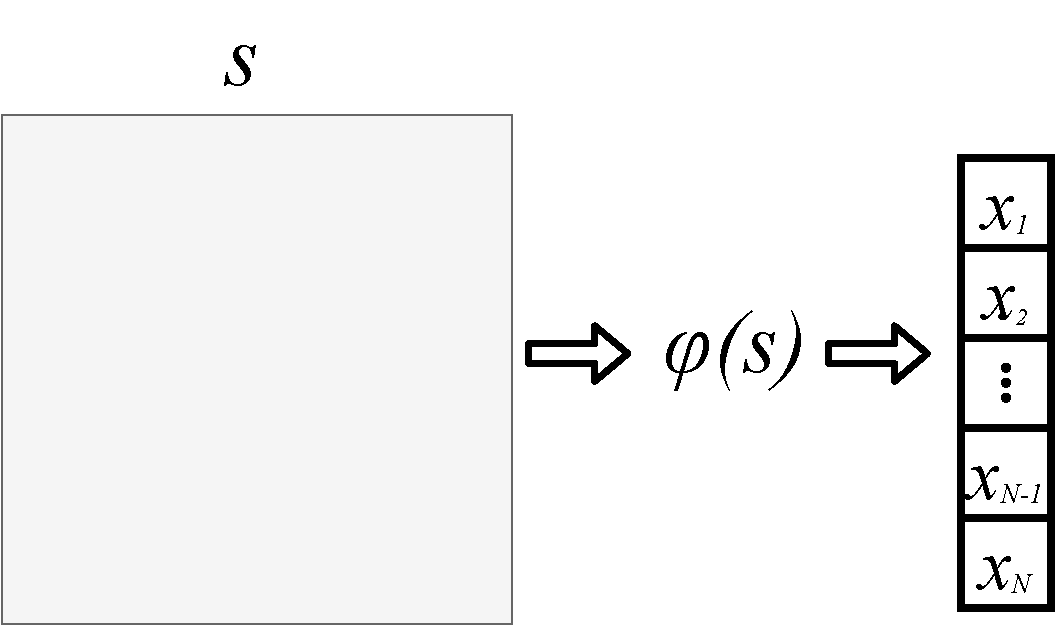
\includegraphics[scale=0.25]{Chapter4/Figs/stox.pdf}
    \caption{La observación $s$ del agente se traduce mediante la función $\phi$ en un vector de variables de alto nivel.}
    \label{fig:obs-to-macro}
\end{figure}

Una vez que se
realiza el mapeo entre el espacio de
estados y el de macro variables, se obtiene una lista  $E$ de variables de interés, las cuales se consultarán en el grafo causal.
Por simplicidad, la lista $E$ se obtiene a través de una función $f$ que calcula cuáles variables tienen un valor diferente entre el vector meta $\mathbf{g}$
y el vector de macro variables $\mathbf{x}$. Se puede suponer que $\mathbf{x} \neq \mathbf{g}$, sin embargo, dado que los ambientes son dinámicos, no se puede asegurar que la configuración inicial de un ambiente no sea igual a la que se desea llegar. 

% A menudo, la meta final de una tarea en RL está compuesta de submetas. Por ejemplo, un brazo robótico cuya meta es mover un objeto de un punto $P_x$ a otro $P_y$, antes debe tomarlo  algunos casos,   
En algunos casos, las variables de interés pueden seguir un orden causal, lo que se puede interpretar como que una meta depende de que se cumplan otras submetas.
Por lo tanto, la lista $E$ puede guardarse en un estructura de datos tal que sus elementos estén ordenados por una función de prioridad, por ejemplo, de acuerdo con el orden topológico de $\mathcal{D}$. Con esto, los elementos con mayor prioridad pueden ser las variables que llevan a cumplir submetas necesarias para alcanzar la meta final.
En la Figura \ref{fig:e-list} se describe un ejemplo de cómo se produce la lista $E$ con respecto al grafo de la Figura \ref{fig:example-d}. 


\begin{figure}[h]
    \centering
    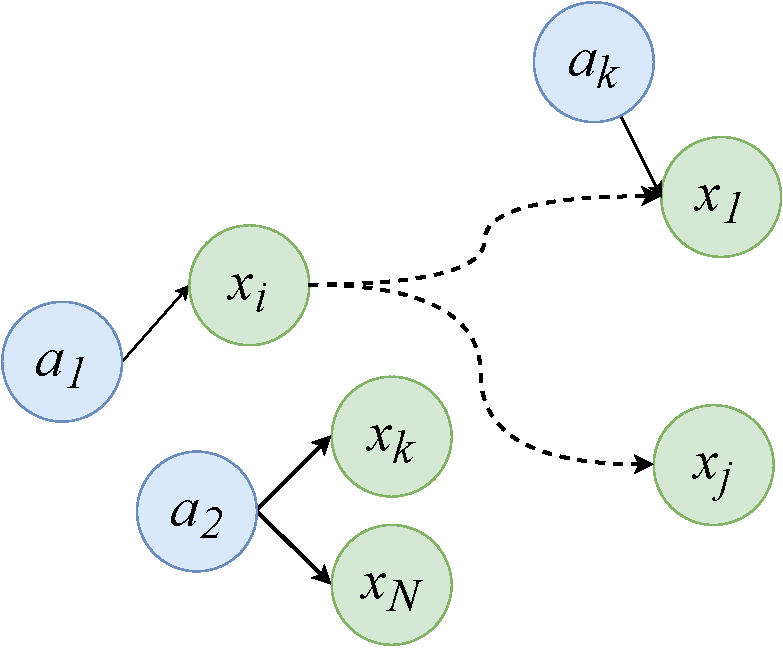
\includegraphics[scale=0.3]{Chapter4/Figs/examplegraph.pdf}
    \caption{Ejemplo de un grafo causal $\mathcal{D}$. Las flechas con cuerpo curvo y punteado denotan caminos causales (notación arbitraria del autor).}
    \label{fig:example-d}
\end{figure} 


\begin{figure}[h]
    \centering
    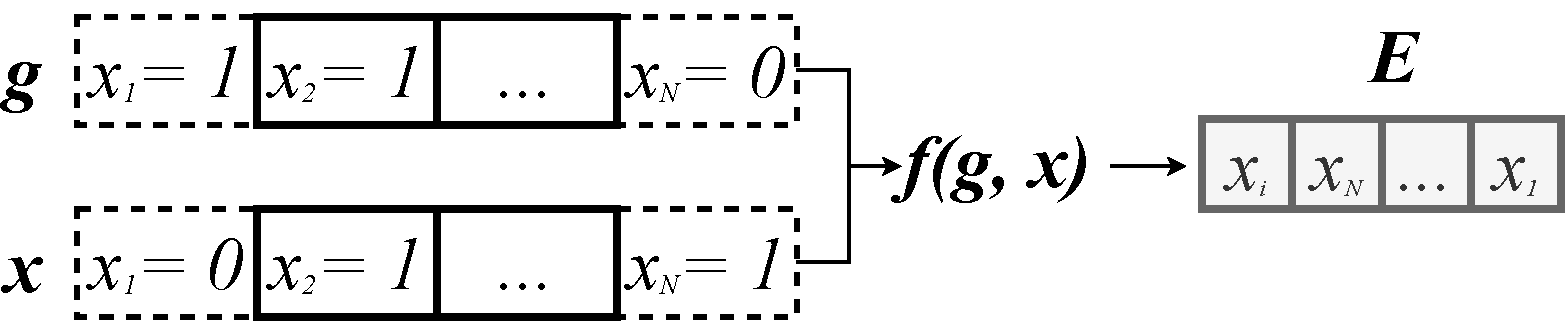
\includegraphics[scale=0.45]{Chapter4/Figs/listofinterest.pdf}
    \caption{La lista $E$ se obtiene de las variables que tienen valores diferentes entre los vectores $\mathbf{x}$ y $\mathbf{g}$. En este ejemplo, se almacenan la variable $x_i$ en $E$ si $|x_i - x_i' | = 1$ tal que $x_i\in \mathbf{g}$ y $x_i' \in \mathbf{x}$. El orden de $E$ sigue el orden topológico de grafo de la Figura \ref{fig:example-d}.}
    \label{fig:e-list}
\end{figure} 

El siguiente paso corresponde a obtener una acción $a \in \mathcal{A}$ para que el agente la lleve a cabo.
Para esto, se hace un recorrido sobre la lista $E$, donde
por cada elemento $e \in E$ se hace una consulta al grafo causal. La consulta consiste en la
obtención de los padres de $e$.  Si $e$ se encuentra en el grafo y además tiene al menos una variable de acción $a$ como predecesor se realiza tal acción.
En este trabajo, solo se abordan problemas donde los grafos causales solo tienen conexiones donde la acciones son vértices sin padres y además no es necesario llevar a cabo varias acciones al mismo tiempo para afectar a $e$.
% Algunos posibles casos de los tipos de conexiones entre las acciones y las variables de interés se pueden ver en la Figura \ref{fig:connection-types}. 
% Las conexiones (a) representan el caso donde una variable de estado $e'$ afecta la acción que se desea tomar.
% % El grafo (b) denota el caso donde para llevar a cabo una acción $a$ es necesario realizar antes la acción $a'$. La estructura (c) muestra el caso donde $e$ solo es afectado cuando varias acciones son ejecutadas al mismo tiempo (el autor añade arbitrariamente una conexión entre las aristas para diferenciar este caso del (d)). 
% Finalmente, el caso atacado en este trabajo es (d), donde la acciones son nodos sin padres y además no es necesario llevar a cabo varias acciones al mimo tiempo para cambiar $e$.

% Esta tesis se limita a trabajar en tareas donde las estructuras causales subyacentes solo contienen conexiones del tipo (d) de la Figura \ref{fig:connection-types}.  

% \begin{figure}
%     \centering
%     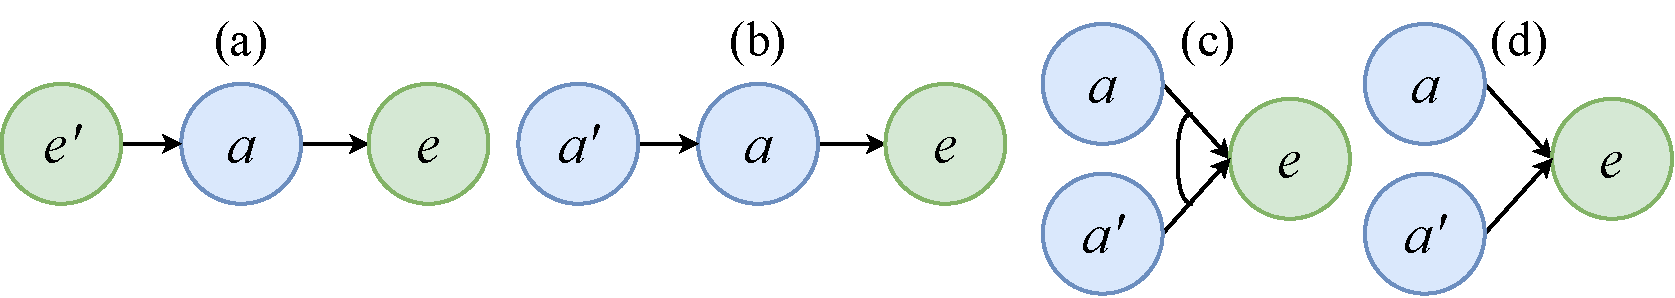
\includegraphics[scale=0.3]{Chapter4/Figs/connections.pdf}
%     \caption{Algunos casos de las conexiones entre la acción $a \in \mathcal{A}$ y la variable de interés $e \in E$. Esta tesis se enfoca en problemas que contienen solo el  caso más simple (d), donde la acción $a$ no depende de que sucedan otras variables $e'$ ni de otras acciones $a'$ (caso (a) y (b), respectivamente). Además, en este tipo de estructuras, no es necesario llevar a cabo más de una acción al mismo tiempo para cambiar el estado de $e$ (caso (c)).}
%     \label{fig:connection-types}
% \end{figure}

% Explicar un poco más esto, como están conectadas estas variables siempre a-x o puede haber algo como a-y-x y el caso de que las causas son independientes entre ellas, tal vez añadir eso en las suposiciones. Como que la x es hija de varias que pasa, tal vez enumerar lo casos
% Caso 1) es una causa directa y no es de efecto común
% caso 2) causa directa y es de efecto común
% caso 3 causa lejana pero no hay más info entonces la ejecuto
% caso 4) o los caoss deben dividirse si son de efecto común o causa común. Este último es complicado porque hacer algo que afecta a otros elementos que no quiero afectar es un problema. Recalcar que casos atacamos
% se regresa una acción aleatoria que es causa directa de esa variable $x_i$. 

% Poner ejemplo, imágenes de los casos? Tal vez solo decir cuál de todas las acciones se selecciona. Enfatizar en que las acciones son independientes. Tal vez una imagen de los posibles casos y además del que se ataca en los dominios propuestos.

% En caso de que no haya información suficiente, es decir, no se encontró ninguna acción realizable, la política regresa una acción aleatoria, por lo que el agente realiza un exploración a ciegas. Para evitar que repetir intentar actuar sobre las variables de interés, aunque tal vez esto no es necesario porque se supone que una vez ya intenté tal acción.
% se obtienen las variables de interés y el orden en que se obtienen las causas de 
% cada variable de interés, se hace un barajado sobre éstas.
% Tal vez todo esto está de más, yo creo que sí por eso de que $E$ está en orden aleatorio ya me quito de todo esto

El método propuesto encaja sin problemas y se incorpora en el algoritmo Q-learning \cite{watkins1992q}. El proceso de entrenamiento 
 del algoritmo Q-learning se mantiene idéntico salvo por  la selección de acciones guiada.
En los Algoritmos
\ref{alg:q-algo-extra-info} y \ref{alg:dqn-algo-causal}, se presentan los métodos resultantes al añadir la selección de acciones guiada, Q-learning clásico y DQN, respectivamente. Además, se puede notar que el proceso de selección de acción propuesto no está atado a un esquema $\epsilon$-greedy. Se podría utilizar otro método basado en política, por ejemplo, donde antes de utilizar la política que se está aprendiendo, se consulte el modelo causal. Sin embargo, explorar otros esquemas de selección queda fuera de este trabajo.

\begin{mialgoritmo}[H]
  	\caption{$Q$-learning guiado por conocimiento causal}
	\label{alg:q-algo-extra-info}
  \begin{algorithmic}[1]
  \setstretch{1}
  \REQUIRE Estructura causal $\mathcal{D}$, la meta $\mathbf{g} = [x_1, \dots, x_n]$ donde $x_i \in \mathcal{X}$, la tasa de aprendizaje $\alpha \in (0,1]$, el número de episodios $k$, el horizonte $H$ de cada episodio, el coeficiente $\delta$, los valores $\epsilon_{\max}$ y $\epsilon_{\min}$.
  \STATE Inicializar arbitrariamente $Q(s,a)$, para todo $s\in \mathcal{S}$ excepto donde $Q(terminal, \cdot) = 0$.
  
  \FOR{$episodio = 1, \dots, k$}
    \STATE Inicializar $s_0$.
    \FOR{$t = 0, \dots, H$}
    \STATE $\epsilon \leftarrow \max(\epsilon_{\min}, \epsilon_{\max} - \frac{|\epsilon_{\max} - \epsilon_{\min}| \times t}{H \times k \times \delta})$.
    \STATE Elegir $a_t$ usando el Algoritmo \ref{alg:guided-action-selection}, que recibe como entrada $\mathcal{D}$, $\mathbf{g}$, $s_t$ y $\epsilon$.
    \STATE Tomar acción $a_t$ y observar $r_{t+1}, s_{t+1}$.
    \STATE $Q(s_t, a_t) \leftarrow Q(s_t, a_t) + \alpha [r_{t+1} + \gamma \max_a Q(s_{t+1}, a) - Q(s_t, a_t)]$.
    \STATE $s_t \leftarrow s_{t+1}$.
    \ENDFOR
  \ENDFOR
  \end{algorithmic}
\end{mialgoritmo}


\begin{mialgoritmo}[H]
  	\caption{DQN guiado por conocimiento causal.}
	\label{alg:dqn-algo-causal}
  \begin{algorithmic}[1]
  \setstretch{1}
  \REQUIRE Estructura causal $\mathcal{D}$, la meta $\mathbf{g} = [x_1, \dots, x_N]$ donde $x_i \in \mathcal{X}$, el número de episodios $k$, el horizonte $H$ de cada episodio, el coeficiente $\delta$, los valores $\epsilon_{\max}$ y $\epsilon_{\min}$.
  \STATE Inicializar búfer de experiencias $D$ con capacidad $M$, la función de valor de acción $Q$ con pesos aleatorios $\theta$ y la función de valor de acción objetivo $\hat{Q}$ con pesos $\theta^- = \theta$.
  
  \FOR{$episodio = 1, \dots, k$}
    \STATE Inicializar $s_0$.
    \FOR{$t = 0, \dots, H$}
    \STATE $\epsilon \leftarrow \max(\epsilon_{\min}, \epsilon_{\max} - \frac{|\epsilon_{\max} - \epsilon_{\min}| \times t}{H \times k \times \delta})$.
    \STATE Elegir $a_t$ usando el Algoritmo \ref{alg:guided-action-selection}, que recibe como entrada $\mathcal{D}$, $\mathbf{g}$, $s_t$ y $\epsilon$.
    \STATE Tomar acción $a_t$, observar recompensa $r_{t}$ e imagen $s_{t+1}$.
    % \STATE Asignar $s_{t+1} =  s_t, a_t, x_{t+1}$ y preprocesar $\phi_{t+1} = \phi(s_{t+1})$.
    \STATE Guardar transición $(s_t, a_t, r_t, s_{t+1})$ en $D$.
    \STATE De $D$ tomar una muestra aleatoria de un lote de transiciones $(s_j, a_j, r_j, s_{j+1})$.
    \STATE Establecer
	\[
	 y_j = 
   \begin{cases} 
      r_j  & \mbox{si el episodio termina en el paso } j + 1 \\
      r_j + \gamma \max_{a'}\hat{Q}(s_{j+1}, a'; \theta^-) & \mbox{en cualquier otro caso.}
   \end{cases}
	\]
	\STATE Realizar el paso del
	descenso de gradiente sobre $(y_j -  Q(s_j,a_j;\theta))^2$ con respecto a los parámetros de la red $\theta$.
	\STATE Cada $C$ pasos reiniciar $\hat{Q} = Q$.
    \ENDFOR
  \ENDFOR
  \end{algorithmic}
\end{mialgoritmo}


\section{Ejemplo: Problema de los interruptores de luz}\label{section:switches-example}

En esta sección se describe un ejemplo sobre un problema en que se realizan 
lo experimentos de esta investigación. Por ahora, solo se describe el problema
y cómo se aplica el método propuesto.

Imagina que construyes un robot llamado Joi, con el propósito de prender o apagar las luces de las habitaciones 
de una casa de acuerdo a como se le comande.
A Joi se le puede dotar de cierto conocimiento previo de la configuración
del cableado de la casa, tal que le ayude a descifrar las correspondencias entre
interruptores de luz y los focos de las habitaciones. 
 A Joi le gusta aprender mediante prueba
 y error y recibir una señal de recompensa positiva o negativa de acuerdo a su comportamiento. Además, el robot 
 necesita repetir muchas veces la misma acción para aprender
 qué provocará realizarla. Por lo tanto, si Joi conoce los efectos de algunas de sus acciones (mover los interruptores), puede reducir sus intentos para
 resolver las conexiones entre interruptores y los focos. 
 Por ejemplo, con anticipación Joi puede saber que el mover interruptor de luz $i$ causa que
prenda o apague la luz de la cocina.
 Así que al darle la orden de prender las luces de la cocina, el baño y de alguna otra habitación, Joi solo se enfoca en aprender las partes que no
 conoce.
 
 El problema se puede ver como una tarea donde es necesario tomar las
 decisiones adecuadas para llegar a un configuración de luces deseada. Formalmente, se puede ver como un MDP condicionado a metas donde 
 
 \begin{itemize}
     \item El espacio de estados $\mathcal{S}$, es el conjunto de
     posibles observaciones de la casa desde una vista cenital como en la Figura
   \ref{fig:obs-switches}.
     \begin{figure}[H]
         \centering
         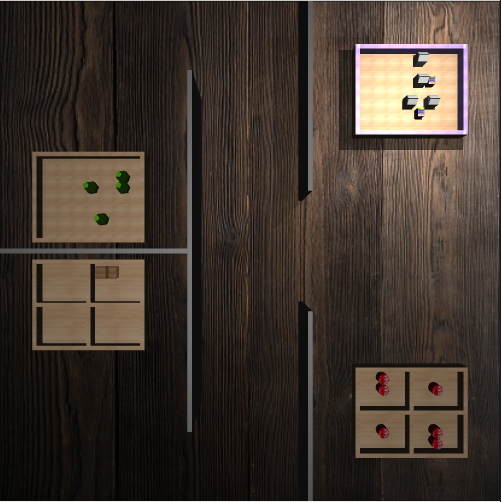
\includegraphics[scale=0.17]{Chapter4/Figs/example_obs.png}
         \caption{Observación disponible para el robot.}
         \label{fig:obs-switches}
     \end{figure}
     \item El espacio de acciones es $\mathcal{A} = \{a_1, a_2, \dots, a_N\}$
     donde cada $a_i$ corresponde a mover o no el interruptor de luz $i$. $a_i = 0$ si no se mueve el interruptor y $a_i = 1$ si se mueve.
     \item El conjunto de variables de alto nivel $\mathcal{X} = \{x_1, x_2, \dots, x_N\}$ contiene
     a las variables que describen el estado de cada foco en la casa. Por ejemplo, $x_i = 1$ establece que el foco $i$ está prendido.
     \item El grafo causal $\mathcal{D} = <\mathcal{A'}, \mathcal{X'}>$, donde
     $\mathcal{A'} \subseteq \mathcal{A}$ y $\mathcal{X'} \subseteq \mathcal{X}$, visualmente el grafo se puede representar como en la Figura \ref{fig:dag-example-switches}.
     
     \begin{figure}[H]
         \centering
         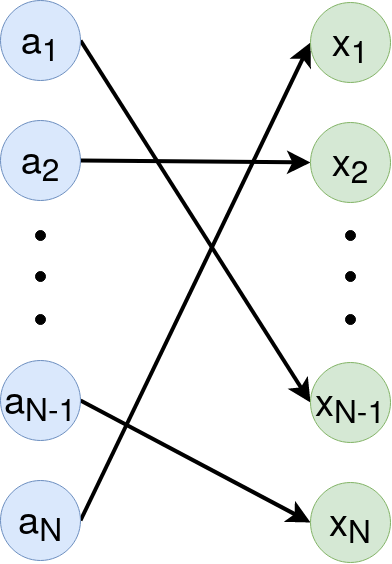
\includegraphics[scale=0.2]{Chapter4/Figs/graph.png}
        \caption{Una estructura causal posible para $N$ interruptores y $N$ luces
        con un tipo de conexión uno-a-uno.}
        \label{fig:dag-example-switches}
     \end{figure}
     \item No se cuenta con la función de transición $\mathcal{P}$, sin embargo,
     se conoce que el interruptor $i$ no necesariamente corresponde al foco $i$.
     \item El espacio de metas $\mathcal{G}$ contiene a todas las
     combinaciones posibles de focos prendidos y apagados en la casa.
     \item La recompensa inmediata $r$ se calcula a través de medir la diferencia entre la observación y la meta.
 \end{itemize}
 
 Una vez que la tarea se ha descrito como un MDP, es posible que Joi
 aprenda a alcanzar una configuración de luces deseada
 utilizando un algoritmo de RL, Q-learning por ejemplo. Además,
 dado que suponemos que Joi puede aprovechar el conocimiento que le
 ofrece el grafo causal $\mathcal{D}$, la selección de acciones se puede
 guiar usando el Algoritmo \ref{alg:guided-action-selection}. 
 En la Figura \ref{fig:example-switches} se muestra un paso en el proceso de aprendizaje.
 
 \begin{figure}
     \centering
     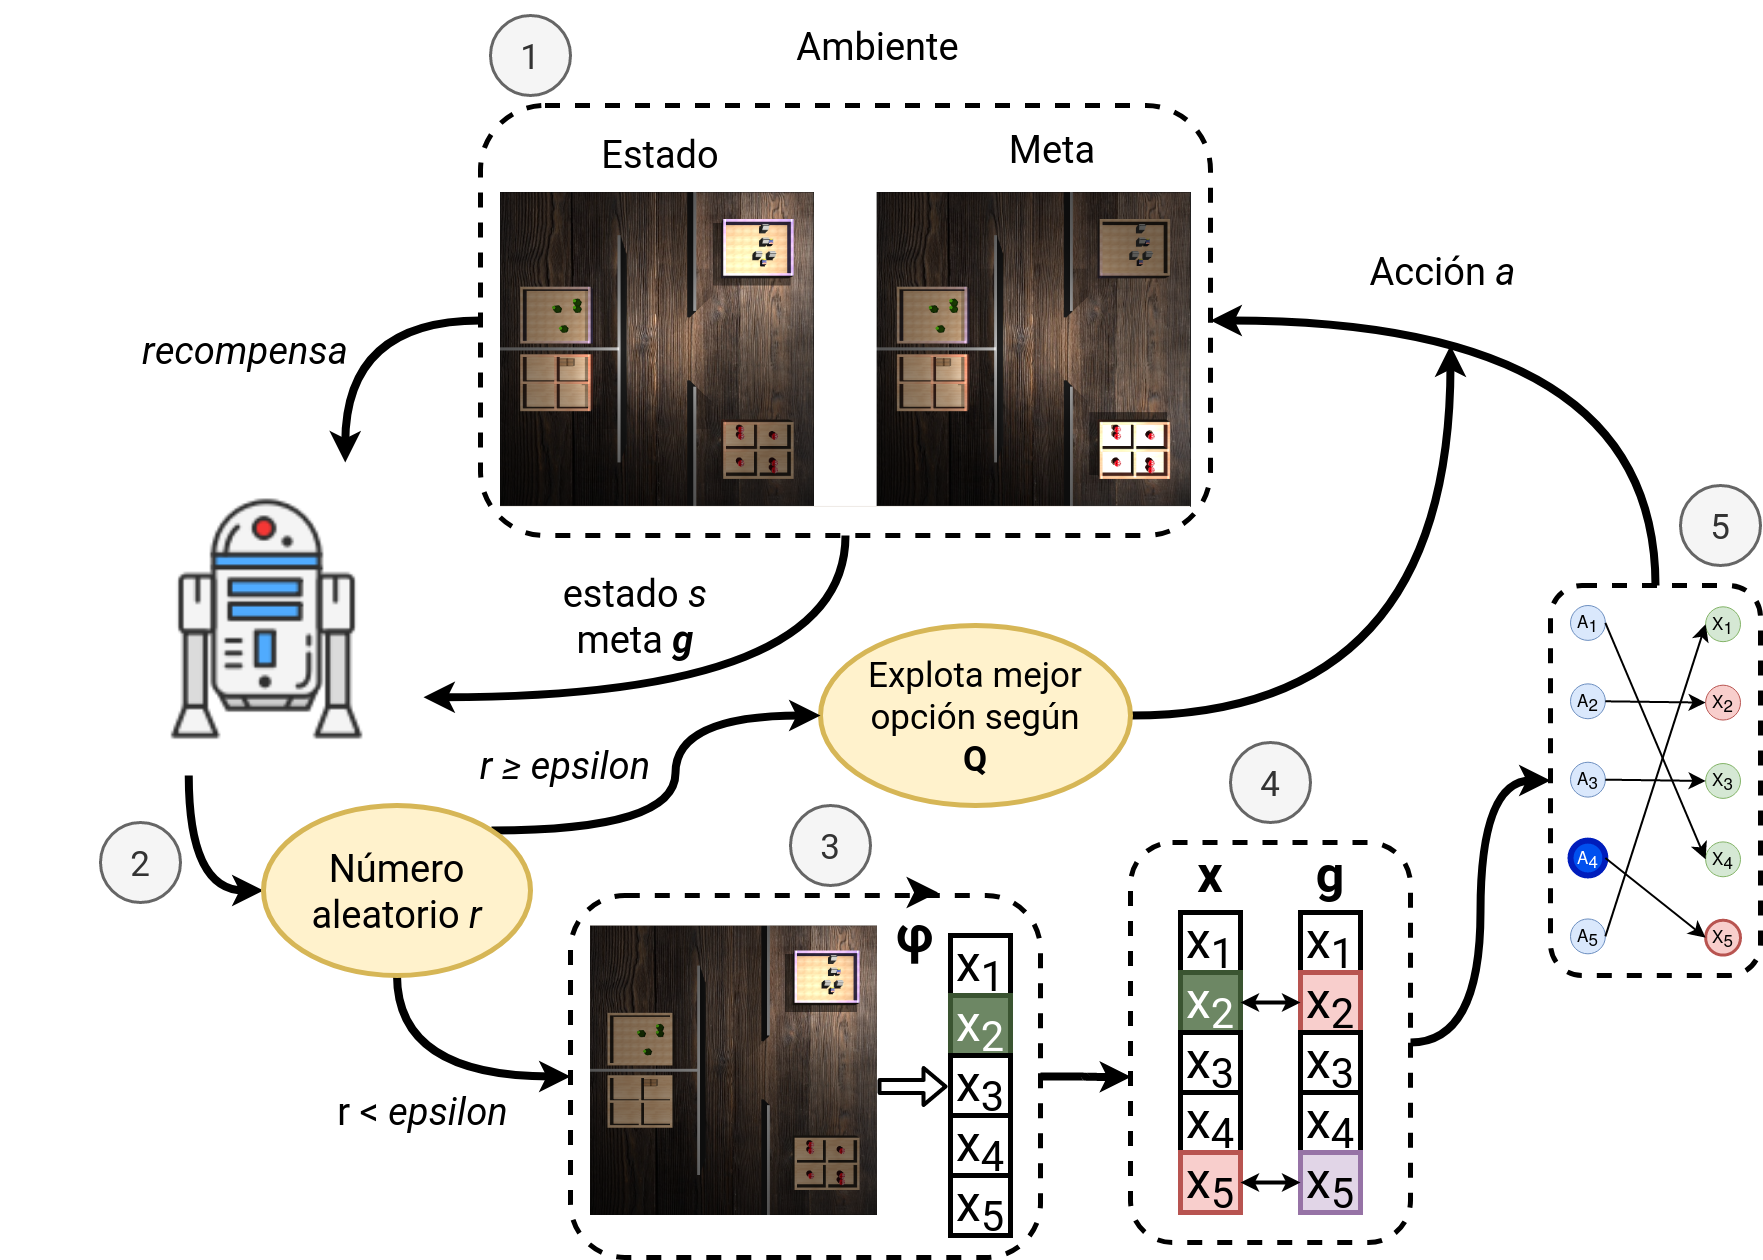
\includegraphics[scale=0.25]{Chapter4/Figs/example_method.png}
     \caption{Interacción del agente con su ambiente: 1) el agente observa el estado de su ambiente además de conocer el vector $\mathbf{g}$, 2) inicia
     la política de selección de acciones, 3) si el agente debe explorar, mapea la observación a un vector de variables de alto nivel $\mathbf{x}$, 4) se calculan los diferentes entre los vectores $\mathbf{x}$ y $\mathbf{g}$, 5) se consultan los padres de las variables de interés y se retorna la acción. El entrenamiento continúa su aprendizaje de manera normal.}
     \label{fig:example-switches}
 \end{figure}
 
 \clearpage
 \section{Resumen}
 
En este capítulo se presentó el tipo de tareas que se 
desean atacar junto con el método propuesto. La propuesta
integra un modelo causal en un algoritmo de aprendizaje por refuerzo para
acelerar su aprendizaje.
Las tareas que se desean atacar, son 
planteadas como procesos de decisión de Markov dirigidos por metas.
La principal característica de este tipo de problemas, que es de interés para este trabajo,
es el contar con una estructura causal del ambiente en un espacio 
que puede ser de menor dimensión que el de las observaciones.
El método propuesto se puede dividir en dos partes, que
corresponden con las contribuciones de este trabajo:

\begin{enumerate}
    \item \textit{Una representación de las relaciones causales del mundo del agente.} Para hacer consultas sobre un modelo causal del ambiente, se utiliza la estructura causal $\mathcal{D}$, la cual tiene como vértices las variables de estado y de acción.
    \item  \textit{Un esquema de interacción entre un algoritmo de aprendizaje por refuerzo
    y un modelo causal}. Se introduce un algoritmo basado en la política de selección
    de acciones $\epsilon$-greedy, el cual guía la elección de acciones de acuerdo
    a las conexiones en el grafo $\mathcal{D}$.
\end{enumerate}
